\documentclass[10pt,a4paper]{article}

\usepackage[utf8]{inputenc}
\usepackage[T1]{fontenc}
\usepackage{lmodern}
\usepackage[english]{babel}
\usepackage[margin=1.5cm,top=1.3cm,bottom=1.6cm]{geometry}
\usepackage{amsmath,amssymb}
\usepackage{booktabs}
\usepackage{graphicx}
\usepackage{listings}
\usepackage[dvipsnames]{xcolor}
\usepackage[most]{tcolorbox}
\usepackage{enumitem}
\usepackage{titlesec}
\usepackage[hidelinks,pdftitle={Assignment 2 - Cheat Sheet},pdfauthor={},pdfcreator={},pdfproducer={}]{hyperref}
\pdfstringdefDisableCommands{\def\code#1{#1}}

\graphicspath{{../plotting/}}

\setlength{\parindent}{0pt}
\setlength{\parskip}{3pt}
\setlength{\emergencystretch}{2em}
\setlist{nosep,leftmargin=1.3em}

\definecolor{blau}{HTML}{2A78D6}
\definecolor{orange}{HTML}{EB6834}
\definecolor{grau}{HTML}{F3F5F8}

\titleformat{\section}{\Large\bfseries\color{blau}}{}{0pt}{}[\vspace{-2pt}{\color{blau}\titlerule[0.8pt]}]
\titleformat{\subsection}{\large\bfseries}{}{0pt}{}
\titlespacing*{\section}{0pt}{9pt}{4pt}
\titlespacing*{\subsection}{0pt}{8pt}{3pt}
\makeatletter
\newcommand{\secneed}[1]{\par\penalty\@M\begingroup\setlength{\dimen@}{#1}\dimen@ii\pagegoal
  \advance\dimen@ii-\pagetotal\ifdim\dimen@>\dimen@ii\ifdim\dimen@ii>\z@\vfil\fi\penalty-\@M\fi\endgroup}
\makeatother
\let\oldsection\section
\renewcommand{\section}{\secneed{9\baselineskip}\oldsection}

\lstset{
  language=C++,
  basicstyle=\ttfamily\footnotesize,
  keywordstyle=\color{blau}\bfseries,
  commentstyle=\color{gray}\itshape,
  numbers=left,
  numberstyle=\tiny\color{gray},
  numbersep=6pt,
  backgroundcolor=\color{grau},
  frame=leftline,
  rulecolor=\color{blau},
  framerule=2pt,
  xleftmargin=18pt,
  columns=fullflexible,
  keepspaces=true,
  showstringspaces=false,
  aboveskip=4pt,
  belowskip=2pt
}

\newtcolorbox{fragen}{
  enhanced, breakable, colback=orange!6, colframe=orange, boxrule=0.6pt, arc=2pt,
  left=6pt, right=6pt, top=4pt, bottom=4pt,
  title={\bfseries Likely questions}, coltitle=white, fonttitle=\bfseries, fontupper=\small
}
\newtcolorbox{herleitung}[1]{
  enhanced, breakable, colback=blau!6, colframe=blau, boxrule=0.6pt, arc=2pt,
  left=6pt, right=6pt, top=4pt, bottom=4pt,
  title={\bfseries Derivation: #1}, coltitle=white, fonttitle=\bfseries
}
\newtcolorbox{extra}{
  enhanced, breakable, colback=gray!7, colframe=gray!70!black, boxrule=0.6pt, arc=2pt,
  left=6pt, right=6pt, top=4pt, bottom=4pt,
  title={\bfseries With orientation included -- short version is in the report (A5 b, determinant)},
  coltitle=white, fonttitle=\bfseries, fontupper=\small
}

\tcbset{before skip=5pt, after skip=5pt}

\newcommand{\frage}[2]{\textbf{Q: #1}\par\nopagebreak\vspace{1pt}\textbf{A:} #2\par\vspace{5pt}}
\newcommand{\sagen}[1]{\textbf{In short:} \emph{#1}\par}
\newcommand{\code}[1]{\texttt{#1}}

\begin{document}
\small

{\LARGE\bfseries Assignment 2 -- Cheat sheet for the presentation}\par
\vspace{2pt}
{\large Code from \code{forwardkinematics.cpp} and \code{control.cpp}, gains from \code{gains\_1.txt},
numbers from the report}

%=====================================================================
\section{At a glance}
%=====================================================================

{\small\setlength{\tabcolsep}{4pt}
\begin{tabular}{@{}llll@{}}
  \toprule
  Task & Function & What happens & Result \\
  \midrule
  A1 & \code{computeDH} & DH table (Craig) & $\theta_2 = q_2 - \frac{\pi}{2}$, otherwise only $L_1, L_2, L_3$ \\
  A2 & \code{computeT0\_1} \ldots{} \code{computeT0\_E} & Transformations & ${}^0_ET$ simplified, $(x, y)$ at $q = 0$: $(0.41, -0.49)$ \\
  A3 & \code{computeF} & $F = (x, y, \alpha)$ & $\alpha = q_1 + q_2 + q_3 - \frac{\pi}{2}$, at $q = 0$: $\alpha = -1.57$ \\
  A4 & \code{computeJ} & $J = \partial F / \partial q$ & last row $(1, 1, 1)$ \\
  A5 & Sketch & Columns of $J$ as arrows & i controllable, ii close to, iii in singularity \\
  B1 & Calculation & 2 cubic splines + via point & $\dot q_b = (-0.31,\ 0,\ 0)$\,rad/s \\
  B2 & \code{computeTf}, \code{computeSpline}, \code{followSpline} & Spline + PD + $G$ & proj1: $t_f = 2.47$\,s, error $< 0.01$\,rad \\
  C1 & \code{setCircleTarget}, \code{proj2Control} & Circle, $\beta = \dot\beta\,t$ & 5\,s per circle, $0.25$\,m/s \\
  C2 & \code{operationalSpaceControl} & $\tau = J^T F + G$ & no inverse kinematics \\
  C3 & Gains & Error $\sim 1/k_p$ & max.\ 11\,mm, RMS 7\,mm, $\tau_1$ up to 116\,Nm \\
  C4 & \code{proj3Control} & Parabolic blends for $\beta$ & $t_b = 5$\,s, $t_f = 20$\,s, $\tau_1$ up to 68\,Nm \\
  C5 & \code{line}, \code{xtrack}, \code{nxtrack}, \code{ntrack} & Bonus & max.\ circle 11, line 22, square 50\,mm \\
  \bottomrule
\end{tabular}
}

\subsection{Gains and numbers}
{\small
\begin{tabular}{@{}lll@{}}
  \toprule
  Controller (number in the \code{kp}/\code{kv} command) & $k_p$ & $k_v$ \\
  \midrule
  \code{njtrack} (11), \code{proj1} (21) & $3000 / 1350 / 300$ (joints) & $245 / 70 / 21$ \\
  \code{proj2} (22), \code{proj3} (23) & $8000 / 8000 / 200$ ($x, y, \alpha$) & $280 / 280 / 10$ \\
  Bonus: \code{nxtrack} (13), \code{xtrack} (14), \code{ntrack} (17), \code{line} (20) & same as \code{proj2} & same as \code{proj2} \\
  \bottomrule
\end{tabular}
}

\begin{itemize}
  \item $L_1 = 0.41$\,m, $L_2 = 0.43$\,m, $L_3 = 0.055$\,m (\code{l1}, \code{l2}, \code{l3} in the header). Abbreviations as
        in the report: $s_1 = \sin q_1$, $c_{12} = \cos(q_1 + q_2)$, $s_{123} = \sin(q_1 + q_2 + q_3)$ etc.
  \item Simulator: $\dot q_{\max} = \frac{\pi}{4} = 0.79$\,rad/s, $\ddot q_{\max} = \frac{\pi}{3} = 1.05$\,rad/s$^2$ for all joints,
        $\tau_{\max} = 156.4 / 89.4 / 20.1$\,Nm.
\end{itemize}

\subsection{Two coordinate frames}
\begin{minipage}[t]{0.49\textwidth}
\textbf{Fig.~1 (part A, \code{forwardkinematics.cpp})}
\begin{itemize}
  \item $x_0$ right, $y_0$ \textbf{down}, $z_0$ into the page.
  \item Positive angles = \textbf{clockwise} in the figure.
  \item Zero configuration: link 1 horizontal to the right, links 2 and 3 pointing straight up.
  \item End effector at the top $\Rightarrow$ $y < 0$ and $\alpha = -\frac{\pi}{2}$.
\end{itemize}
\end{minipage}\hfill
\begin{minipage}[t]{0.49\textwidth}
\textbf{Simulator (part C, \code{gv.x})}
\begin{itemize}
  \item $x$ right, $y$ \textbf{up}, $z$ out of the screen.
  \item $\alpha = 0$ means upright. The sheet says: $y$ is the opposite of Fig.~1.
  \item In part C we only use values from the simulator (\code{gv.x}, \code{gv.dx}, \code{gv.Jtranspose}, \code{gv.G}),
        so there is no conversion in the code.
\end{itemize}
\end{minipage}

\vspace{2pt}
(Observation in the simulator: at $q = 0$, \code{gv.x} shows $(0.41,\ 0.59,\ 0)$. So do not compare $F$ from part A
directly with \code{gv.x}, the origin is a different one.)

\subsection{Demo in the simulator (console \code{CS225A:>})}
\begin{enumerate}
  \item 3-DOF mode: \code{robottype 1}. In the GUI switch ``torque limits'' off and click ``Load gains''
        (\code{loadgains} does not work in the console; there use e.g.\ \code{kp 21 3000 1350 300}, \code{kv 21 245 70 21}).
  \item \code{proj1 0 0 0} -- moves to the circle start $(0.8,\ 0.35)$ in 2.47\,s, then float. The three numbers are
        ignored, but the console wants three arguments.
  \item \code{proj2} -- circle, 5\,s per circle, keeps going until another controller is started. (If the console says
        ``expected \ldots{} args'', add zeros as for proj1.)
  \item \code{proj1 0 0 0}, then \code{proj3} -- three circles in 20\,s, smooth start and stop, then holds the end point.
  \item Bonus, each after \code{proj1 0 0 0}: \code{line 0 0 0}, \code{xtrack 0 0 0 0}, \code{nxtrack 0 0 0 0},
        \code{ntrack 0 0 0}.
  \item \code{njtrack}: enter the goal angles in the GUI and start, the arm moves there on a spline.
\end{enumerate}
The console only handles about one command per second, so type slowly.

%=====================================================================
\section{A1: DH parameters}
%=====================================================================

\begin{center}
\begin{tabular}{ccccc}
  \toprule
  $i$ & $\alpha_{i-1}$ & $a_{i-1}$ & $d_i$ & $\theta_i$ \\
  \midrule
  1    & 0 & 0     & 0 & $q_1$ \\
  2    & 0 & $L_1$ & 0 & $q_2 - \frac{\pi}{2}$ \\
  3    & 0 & $L_2$ & 0 & $q_3$ \\
  4(E) & 0 & $L_3$ & 0 & 0 \\
  \bottomrule
\end{tabular}
\end{center}
\vspace{-6pt}
\begin{itemize}
  \item $\boldsymbol{\alpha = 0}$: the arm is planar, all $z$ axes are parallel. $\boldsymbol{d = 0}$: all frames are in
        one plane, no shift along $z$.
  \item $\boldsymbol{a_{i-1}}$: distance between the joint axes = link length. $a_0 = 0$, because frames 0 and 1 are at
        the same point.
  \item $\boldsymbol{\theta_i}$: all joints are revolute, so $q_i$ is in $\theta_i$. $\theta_4 = 0$: there is no joint
        between frame 3 and E.
\end{itemize}

\textbf{Theory in two sentences (tutorial, Craig):} The DH convention describes the transformation between two frames
with only four numbers. $\alpha_{i-1}$ and $a_{i-1}$ belong to the $x$ axis (angle and distance between two $z$ axes),
$d_i$ and $\theta_i$ to the $z$ axis (distance and angle between two $x$ axes); for a revolute joint $q_i$ is in
$\theta_i$.

\textbf{The $-\frac{\pi}{2}$ in row 2:} $\theta_2$ is the angle from $x_1$ to $x_2$ about $z_2$. In the zero configuration
$x_1$ points right, but $x_2$ points up. So the frames are already rotated against each other when $q_2 = 0$. $z$ points
into the page, positive angles are clockwise. From ``right'' to ``up'' is counter-clockwise, so $-\frac{\pi}{2}$. Between
$x_2$ and $x_3$ (both up) there is no offset.

\secneed{2\baselineskip}
\begin{lstlisting}[firstnumber=112]
const float HALF_PI = 1.57079633f;
\end{lstlisting}
\vspace{-4pt}
\secneed{6\baselineskip}
\begin{lstlisting}[firstnumber=418]
   //row vector: frame 2
   DH[1][0] = 0.0;
   DH[1][1] = l1;
   DH[1][2] = 0.0;
   DH[1][3] = angles[1] - HALF_PI;
\end{lstlisting}
\textbf{L.\,112, 410--435:} Each row of \code{DH} is one row of the table, in the order
$(\alpha_{i-1}, a_{i-1}, d_i, \theta_i)$. \code{HALF\_PI} is our own constant, because we may not use additional
includes.

\sagen{All axes are parallel, so $\alpha$ and $d$ are zero everywhere. What is left are the link lengths in $a$ and the
joint angles in $\theta$, plus a fixed offset of $-\frac{\pi}{2}$ at joint 2, because link 1 is horizontal and link 2 is
vertical.}

\begin{fragen}
\frage{Why $-\frac{\pi}{2}$ and not $+\frac{\pi}{2}$?}
{$y_0$ points down, so $z$ points into the page, and positive angles are clockwise. From $x_1$ (right) to $x_2$ (up) is a
counter-clockwise turn, which is negative. You can check it with $q = 0$: the result is $(0.41, -0.49)$, the end effector
is at the top, as in Fig.~1.}
\frage{Is the DH table unique?}
{Not in general (tutorial): the direction of $z$ is free, for parallel axes the origin along the axis is free, and for
intersecting axes there are two directions for $x$. Here Fig.~1 fixes the frames, and for these frames the table is
unique.}
\frage{Why does frame 0 coincide with frame 1?}
{That is how frame 0 is placed by convention (tutorial, step 7): same origin, same $z$ axis. Then
$\alpha_0 = a_0 = d_1 = 0$, so as many zeros as possible, and ${}^0_1T$ is a pure rotation by $q_1$. That is why Fig.~1
says $x_{0,1}$, $y_{0,1}$.}
\end{fragen}

%=====================================================================
\section{A2: Transformations and forward kinematics}
%=====================================================================

\textbf{Original (tutorial, Craig p.~74)} and \textbf{simplified} with $\alpha_{i-1} = 0$, $d_i = 0$
($c\alpha = 1$, $s\alpha = 0$):
\[
  {}^{i-1}_{\;\;i}T =
  \begin{pmatrix}
    c\theta_i & -s\theta_i & 0 & a_{i-1} \\
    s\theta_i\, c\alpha_{i-1} & c\theta_i\, c\alpha_{i-1} & -s\alpha_{i-1} & -s\alpha_{i-1}\, d_i \\
    s\theta_i\, s\alpha_{i-1} & c\theta_i\, s\alpha_{i-1} & c\alpha_{i-1} & c\alpha_{i-1}\, d_i \\
    0 & 0 & 0 & 1
  \end{pmatrix}
  \;\Rightarrow\;
  \begin{pmatrix}
    c\theta_i & -s\theta_i & 0 & a_{i-1} \\
    s\theta_i & c\theta_i & 0 & 0 \\
    0 & 0 & 1 & 0 \\
    0 & 0 & 0 & 1
  \end{pmatrix}
\]
So only a rotation about $z$ by $\theta_i$ and a shift by $a_{i-1}$ along $x$. For row 2 the
\textbf{shift identities} $\cos(q_2 - \frac{\pi}{2}) = s_2$, $\sin(q_2 - \frac{\pi}{2}) = -c_2$:
\[
  {}^0_1T = \begin{pmatrix} c_1 & -s_1 & 0 & 0 \\ s_1 & c_1 & 0 & 0 \\ 0&0&1&0 \\ 0&0&0&1 \end{pmatrix}
  \quad
  {}^1_2T = \begin{pmatrix} s_2 & c_2 & 0 & L_1 \\ -c_2 & s_2 & 0 & 0 \\ 0&0&1&0 \\ 0&0&0&1 \end{pmatrix}
  \quad
  {}^2_3T = \begin{pmatrix} c_3 & -s_3 & 0 & L_2 \\ s_3 & c_3 & 0 & 0 \\ 0&0&1&0 \\ 0&0&0&1 \end{pmatrix}
  \quad
  {}^3_ET = \begin{pmatrix} 1 & 0 & 0 & L_3 \\ 0 & 1 & 0 & 0 \\ 0&0&1&0 \\ 0&0&0&1 \end{pmatrix}
\]
\textbf{Chain} ${}^0_ET = {}^0_1T\,{}^1_2T\,{}^2_3T\,{}^3_ET$, multiplied step by step and simplified with the
\textbf{angle sum identities} $s_{12} = s_1 c_2 + c_1 s_2$, $c_{12} = c_1 c_2 - s_1 s_2$ (the same for $123$). All
rotations are about the same $z$ axis, so the angles add up to $q_1 + q_2 + q_3 - \frac{\pi}{2}$. The position is the sum
of the three link vectors:
\[
  \boxed{
  {}^0_ET(q) =
  \begin{pmatrix}
    s_{123} & c_{123} & 0 & L_1 c_1 + L_2 s_{12} + L_3 s_{123} \\
    -c_{123} & s_{123} & 0 & L_1 s_1 - L_2 c_{12} - L_3 c_{123} \\
    0 & 0 & 1 & 0 \\
    0 & 0 & 0 & 1
  \end{pmatrix}}
\]

\secneed{5\baselineskip}
\begin{lstlisting}[firstnumber=314]
   T0_E[0][0] = s123;
   T0_E[0][1] = c123;
   T0_E[0][2] = 0.0;
   T0_E[0][3] = l1 * c1 + l2 * s12 + l3 * s123;
\end{lstlisting}
\textbf{L.\,304--336:} \code{computeT0\_E} writes the simplified matrix directly (here the first row), it does not
multiply. \code{c1}, \code{s12}, \code{c123}, \ldots{} (l.\,306--311) are sine and cosine of the angle sums. The four
single matrices are in \code{computeT0\_1} to \code{computeT3\_E} (l.\,136--279), with the derivation in the comment.

\textbf{Checks:} $q = 0$: $(0.41,\ -0.49)$, end effector at the top. $q = (0, \frac{\pi}{2}, 0)$: $(0.90,\ 0)$, rotation =
identity, arm stretched out along $x_0$. $q = (\frac{\pi}{4}, -\frac{\pi}{4}, \frac{\pi}{4})$: $(0.33,\ -0.18)$.

\sagen{Every matrix is only a rotation about $z$ plus a shift along $x$. Because all of them rotate about the same axis,
the angles add up, and the position is the sum of the three links.}

\begin{fragen}
\frage{Did you simplify? What was the original equation?}
{Yes. The original is the general DH matrix above. First we put in $\alpha = 0$, $d = 0$, then for row 2 the shift
identities, and when multiplying the angle sum identities. So the result only contains $s_{12}$, $c_{123}$ etc.}
\frage{Why is $y$ negative in the zero configuration?}
{Because $y_0$ points down in Fig.~1. The end effector is $L_2 + L_3 = 0.49$\,m above joint 2, so at $y = -0.49$.}
\frage{How do you know the simplified form is correct?}
{From the checks above (configurations with multiples of $\frac{\pi}{4}$, as the sheet asks). We also compared
${}^0_ET$ with the product of the four matrices in our own test.}
\end{fragen}

%=====================================================================
\section{A3: End effector position \texorpdfstring{$F(q)$}{F(q)}}
%=====================================================================

$x$ and $y$ are in the last column of ${}^0_ET$. $\alpha$ is the angle from $x_0$ to $x_E$. The first column of the
rotation is $x_E$ in frame 0, so $(s_{123}, -c_{123})$. Compare with $(\cos\alpha, \sin\alpha)$:
\[
  \cos\alpha = s_{123},\quad \sin\alpha = -c_{123} \;\Rightarrow\; \alpha = q_1 + q_2 + q_3 - \frac{\pi}{2}
  \qquad
  \boxed{F(q) = \begin{pmatrix}
    L_1 c_1 + L_2 s_{12} + L_3 s_{123} \\
    L_1 s_1 - L_2 c_{12} - L_3 c_{123} \\
    q_1 + q_2 + q_3 - \frac{\pi}{2}
  \end{pmatrix}}
\]
This is also the sum of all $\theta_i$ in the DH table. Checks: $F(0) = (0.41, -0.49, -1.57)$,
$F(0, \frac{\pi}{4}, 0) = (0.76, -0.35, -0.79)$.

\secneed{7\baselineskip}
\begin{lstlisting}[firstnumber=351]
void ForwardKinematicsPuma2D::computeF()
{
   F[0] = T0_E[0][3]; //x
   F[1] = T0_E[1][3]; //y
   F[2] = angles[0] + angles[1] + angles[2] - HALF_PI; //alpha
}
\end{lstlisting}

\sagen{Position from the last column, angle from the first column of the rotation. In the zero configuration the end
effector points up, and ``up'' is $-\frac{\pi}{2}$ in Fig.~1, because $y_0$ points down.}

\begin{fragen}
\frage{Why does $\alpha$ contain $-\frac{\pi}{2}$?}
{$\alpha$ is the angle between $x_0$ and $x_E$. In the zero configuration $x_E$ points up and $x_0$ points right, that is
$-\frac{\pi}{2}$. Without the term $\alpha$ would not fit the rotation matrix: $\cos\alpha$ must be $s_{123}$, not
$c_{123}$. It is the same offset as $\theta_2$ in the DH table.}
\frage{Why not \code{atan2}?}
{$\operatorname{atan2}(-c_{123}, s_{123})$ gives the same angle (up to multiples of $2\pi$). The sum of the angles is
simpler, and the code comment says that both are the same.}
\frage{In the simulator upright is $\alpha = 0$, for you it is $-\frac{\pi}{2}$. Contradiction?}
{No, these are two frames. Part A works in Fig.~1 ($y$ down), the simulator has $y$ up and counts $\alpha$ from the
vertical. Part C only uses the values of the simulator.}
\end{fragen}

%=====================================================================
\section{A4: Jacobian}
%=====================================================================

$J_{ij} = \partial F_i / \partial q_j$: rows $x, y, \alpha$, columns joint 1, 2, 3. Derivatives with
$\frac{\partial}{\partial q}\sin = \cos$, $\frac{\partial}{\partial q}\cos = -\sin$. $q_1$ is in every term, $q_2$ only in
the terms with 12 and 123, $q_3$ only in 123. That is why the columns get shorter from left to right:
\[
  \boxed{
  J(q) =
  \begin{pmatrix}
    -L_1 s_1 + L_2 c_{12} + L_3 c_{123} & L_2 c_{12} + L_3 c_{123} & L_3 c_{123} \\
    L_1 c_1 + L_2 s_{12} + L_3 s_{123} & L_2 s_{12} + L_3 s_{123} & L_3 s_{123} \\
    1 & 1 & 1
  \end{pmatrix}}
  \qquad
  J(0) = \begin{pmatrix} 0.49 & 0.49 & 0.06 \\ 0.41 & 0 & 0 \\ 1 & 1 & 1 \end{pmatrix}
\]

\secneed{4\baselineskip}
\begin{lstlisting}[firstnumber=383]
   J[0][0] = -l1 * s1 + l2 * c12 + l3 * c123;
   J[0][1] = l2 * c12 + l3 * c123;
   J[0][2] = l3 * c123;
\end{lstlisting}
\textbf{L.\,373--396:} \code{computeJ} writes the matrix row by row (here the $x$ row), the $\alpha$ row
(l.\,393--395) is three times \code{1.0}.

\sagen{Each column says how the end effector moves when only one joint turns. We simply took the derivative of $F$ with
respect to each joint angle.}

\begin{fragen}
\frage{What does one column of $J$ mean?}
{How $x$, $y$ and $\alpha$ move when \emph{only} this joint turns ($\dot x = J\,\dot q$). $J$ is the linearisation of the
forward kinematics in the current configuration (tutorial).}
\frage{Why is the last row $(1, 1, 1)$?}
{$\alpha$ is the sum of the three joint angles (minus a constant). Every joint turns the end effector one to one.}
\end{fragen}

%=====================================================================
\section{A5: Jacobian sketches and singularities}
%=====================================================================

\begin{center}
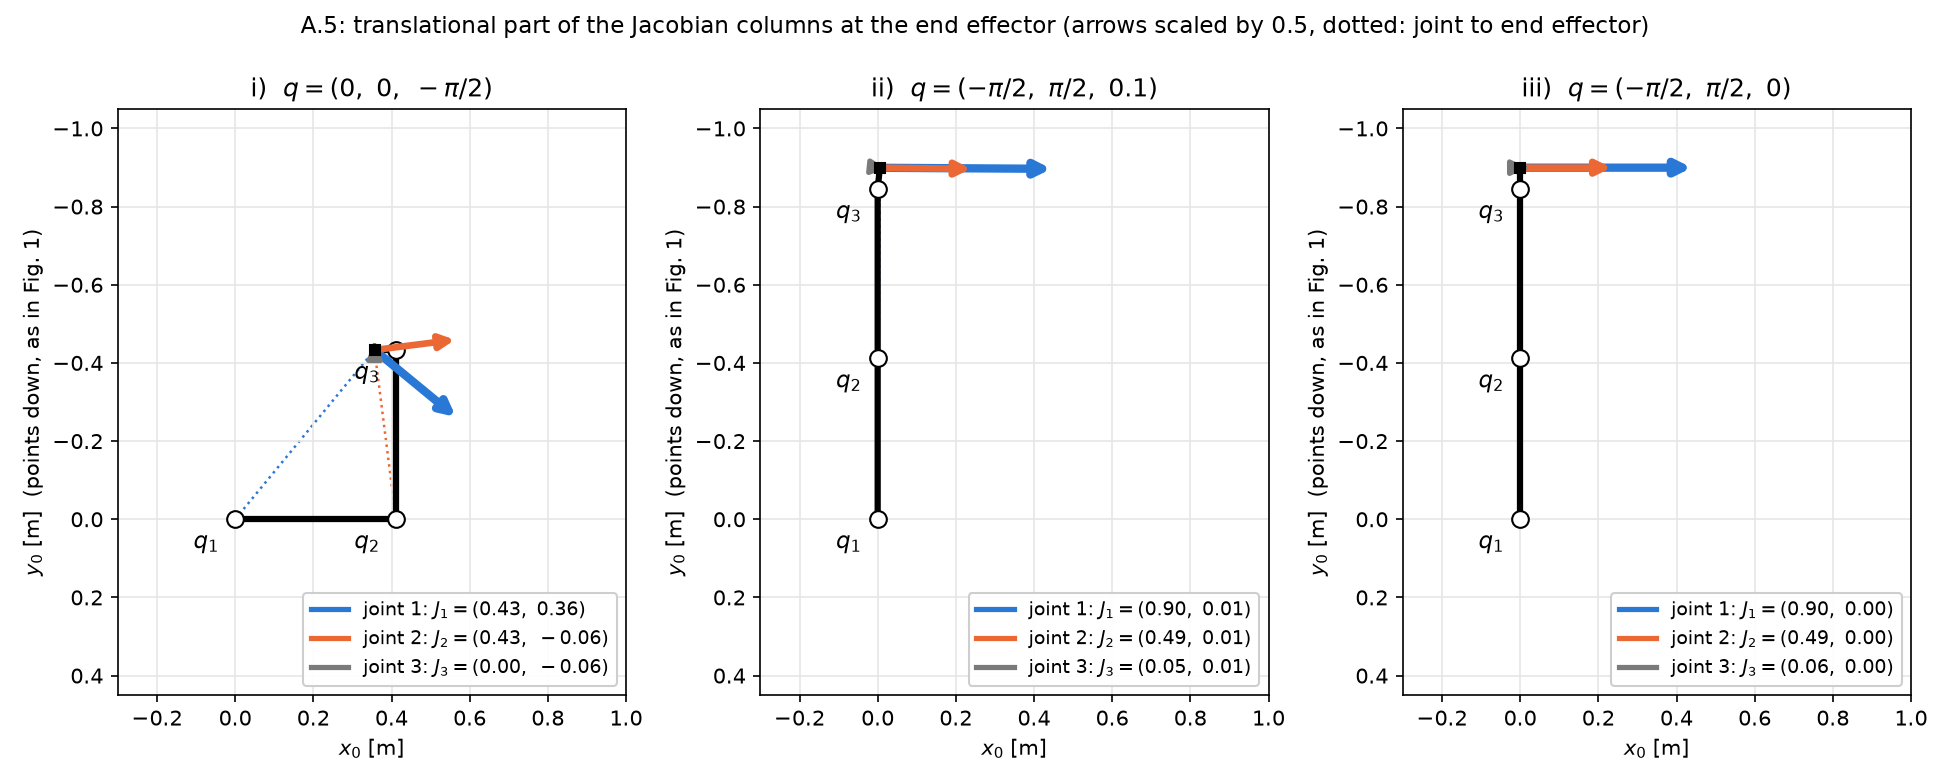
\includegraphics[width=0.72\textwidth]{a5_jacobian.png}
\end{center}
\vspace{-4pt}
\textbf{Drawing the arrows (tutorial):} line from the joint to the end effector (dotted). The arrow is perpendicular to
it, has the same length (drawn at half length in the plot) and points in the direction of a positive rotation, so
clockwise. The numbers are the $x$ and $y$ entries of the columns of $J$.

\begin{itemize}
  \item \textbf{i: fully controllable.} Arrows 1 and 2 point in different directions, together they reach every
        direction. Joint 3 almost only turns the end effector, so it sets the orientation.
  \item \textbf{ii: close to a singularity.} Arm almost stretched out, all arrows almost parallel (sideways). Along the
        arm only $0.01$\,m/rad. Possible, but the joints would have to move very fast.
  \item \textbf{iii: in a singularity.} Arm fully stretched out, all arrows exactly parallel. The end effector cannot move
        along the arm at all, one degree of freedom is lost.
\end{itemize}
\sagen{Different directions = controllable, almost parallel = close to a singularity, exactly parallel = singularity.}

\begin{extra}
$\det J = -L_1 L_2\, c_2$ (subtract column 2 from column 1 and column 3 from column 2, then expand). In ii and iii
$q_2 = \frac{\pi}{2}$, so $\det J = 0$ in \emph{both}. With the orientation included, ii is already singular. The reason:
links 1 and 2 are exactly stretched out. The small motion along the arm in ii only exists because link 3 is turned by $0.1$\,rad. It always comes together with a rotation of the end effector, so $\alpha$ changes too.
The report says both: ``close to'' for the position (sketch, only $x$, $y$) and ``singular'' with the orientation included. In i $q_2 = 0$, $\det J = -L_1 L_2 = -0.18 \ne 0$.
\end{extra}

\begin{fragen}
\frage{How do you see a singularity in the sketch?}
{From the directions of the arrows. If they all point in the same direction (parallel), you cannot combine them into a
motion in the other direction.}
\frage{Why is ii only ``close to'' and iii ``in'' the singularity?}
{In ii the arrows still have a small part along the arm because of $q_3 = 0.1$ ($0.01$\,m/rad), in iii it is exactly zero.
So in ii the motion is still possible, but only with very large joint velocities. This is for the position. With the orientation included ii is already singular as well (see grey box), the report says the same.}
\frage{What happens close to a singularity?}
{A small motion in operational space needs a huge motion in joint space (tutorial T5). We also see it in the bonus: where
$|\det J|$ is small, the error gets larger.}
\end{fragen}

%=====================================================================
\section{B1: Cubic splines with a via point}
%=====================================================================

Two splines per joint: $q_a \to q_b$ ($0$--$2.5$\,s) and $q_b \to q_c$ ($2.5$--$5$\,s), $T = 2.5$\,s, form from the sheet
$q(t) = a_1 + a_2 (t - t_{start}) + a_3 (t - t_{start})^2 + a_4 (t - t_{start})^3$. Four conditions (start and end angle,
start and end velocity) for four parameters, solution from the tutorial:
\[
  a_1 = q_s,\quad a_2 = \dot q_s,\quad
  a_3 = \frac{3}{T^2}(q_e - q_s) - \frac{2}{T}\dot q_s - \frac{1}{T}\dot q_e,\quad
  a_4 = -\frac{2}{T^3}(q_e - q_s) + \frac{1}{T^2}(\dot q_s + \dot q_e)
\]
\textbf{Assumption:} start and end at rest, $\dot q_a = \dot q_c = 0$. \textbf{Heuristic (sheet, Craig):} average
velocities $v_1 = (q_b - q_a)/T = (-0.31,\ 0.63,\ 0)$, $v_2 = (q_c - q_b)/T = (-0.31,\ -0.31,\ 0)$ rad/s.
Joint 1: same sign $\Rightarrow$ average $-0.31$. Joint 2: sign changes $\Rightarrow$ 0. Joint 3: does not move
$\Rightarrow$ 0.

\begin{minipage}[c]{0.5\textwidth}
{\small
\begin{tabular}{ccrrrr}
  \toprule
  Joint & Segment & $a_1$ & $a_2$ & $a_3$ & $a_4$ \\
  \midrule
  1 & $a \to b$ & 0.00    & 0.00    & $-0.25$ & 0.05 \\
  1 & $b \to c$ & $-0.79$ & $-0.31$ & $-0.13$ & 0.05 \\
  2 & $a \to b$ & 0.00    & 0.00    & 0.75    & $-0.20$ \\
  2 & $b \to c$ & 1.57    & 0.00    & $-0.38$ & 0.10 \\
  3 & both      & 0.00    & 0.00    & 0.00    & 0.00 \\
  \bottomrule
\end{tabular}
}
\end{minipage}\hfill
\begin{minipage}[c]{0.47\textwidth}
\textbf{Example} joint 1, first segment:\\
$a_3 = \frac{3}{2.5^2}(-\frac{\pi}{4}) - \frac{-0.31}{2.5} = -0.38 + 0.13 = -0.25$\\
$a_4 = -\frac{2}{2.5^3}(-\frac{\pi}{4}) + \frac{-0.31}{2.5^2} = 0.10 - 0.05 = 0.05$\\
In the plot: the curves go through $q_a, q_b, q_c$, no velocity jump at the via point.
\end{minipage}

\sagen{Two splines per joint that are joined at the via point with the same velocity. The velocity there comes from the
heuristic: direction change 0, otherwise the average.}

\begin{fragen}
\frage{When is the via velocity zero, when is it the average?}
{Per joint: if the direction changes (joint 2 first goes up, then down), it is 0. Otherwise the average of the two
average velocities (joint 1). Joint 3 does not move, so 0.}
\frage{Why cubic and not linear?}
{With linear interpolation the velocity jumps at the start and at the end, which would mean infinite acceleration
(tutorial). With cubic splines we can set the velocity at both ends, so it is also continuous at the via point.}
\frage{The sheet calls the parameters $a_1 \ldots a_4$, the code $a_0 \ldots a_3$?}
{Same thing, only shifted by one. B1 uses the notation of the sheet, B2 the one of the \code{CubicSpline} struct.}
\end{fragen}

%=====================================================================
\section{B2: Spline in joint space (\code{njtrack}, \code{proj1})}
%=====================================================================

At the start \code{initNjtrackControl} computes a spline from \code{gv.q} to \code{gv.qd}, start and end at rest.
With $\Delta q = q_d - q(t_0)$ (tutorial):
$a_0 = q(t_0)$, $a_1 = 0$, $a_2 = \frac{3}{t_f^2}\Delta q$, $a_3 = -\frac{2}{t_f^3}\Delta q$.

\begin{herleitung}{\texorpdfstring{$t_f$}{tf} from the limits (important)}
Derivatives ($t$ counted from $t_0$):
\[
  \dot q_d(t) = 2a_2 t + 3a_3 t^2 = \frac{6\Delta q}{t_f^2}\,t - \frac{6\Delta q}{t_f^3}\,t^2, \qquad
  \ddot q_d(t) = 2a_2 + 6a_3 t = \frac{6\Delta q}{t_f^2} - \frac{12\Delta q}{t_f^3}\,t
\]
The velocity is a \textbf{parabola}, largest in the middle at $t = t_f/2$. The acceleration is a \textbf{straight line},
largest at the start ($t = 0$) and at the end:
\[
  |\dot q|_{\max} = \frac{3|\Delta q|}{2t_f} \le \dot q_{\max} \Rightarrow t_f \ge \frac{3|\Delta q|}{2\dot q_{\max}},
  \qquad
  |\ddot q|_{\max} = \frac{6|\Delta q|}{t_f^2} \le \ddot q_{\max} \Rightarrow t_f \ge \sqrt{\frac{6|\Delta q|}{\ddot q_{\max}}}
\]
$t_f$ = largest of these values over all joints. proj1 from the zero configuration:

\centering
{\small
\begin{tabular}{lccc}
  \toprule
  & Joint 1 & Joint 2 & Joint 3 \\
  \midrule
  $|\Delta q|$ [rad] & 0.10 & 0.97 & 1.06 \\
  $t_f$ from the velocity limit [s] & 0.18 & 1.85 & 2.03 \\
  $t_f$ from the acceleration limit [s] & 0.74 & 2.35 & \textbf{2.47} \\
  \bottomrule
\end{tabular}
}
\end{herleitung}

\secneed{11\baselineskip}
\begin{lstlisting}[firstnumber=41]
double computeTf(GlobalVariables& gv)
{
  double tf = 0.0;
  for (int i = 0; i < gv.dof; i++) {
    double distance = fabs(gv.qd[i] - gv.q[i]);
    double tf_velocity = 1.5 * distance / gv.dqmax[i];
    double tf_acceleration = sqrt(6.0 * distance / gv.ddqmax[i]);
    tf = max(tf, max(tf_velocity, tf_acceleration));
  }
  return tf;
}
\end{lstlisting}
\textbf{L.\,41--51:} Both limits from the derivation for every joint, \code{1.5} $= \frac{3}{2}$. \code{max} keeps the
largest value. The limits come from \code{gv.dqmax} and \code{gv.ddqmax}, not hard-coded.

\secneed{10\baselineskip}
\begin{lstlisting}[firstnumber=58]
  spline.t0 = gv.curTime;
  spline.tf = computeTf(gv);

  PrVector distance = gv.qd - gv.q;
  spline.a0 = gv.q;
  spline.a1 = PrVector(gv.dof);
  if (spline.tf > 0.0) {
    spline.a2 = distance * (3.0 / (spline.tf * spline.tf));
    spline.a3 = distance * (-2.0 / (spline.tf * spline.tf * spline.tf));
\end{lstlisting}
\textbf{L.\,24--31, 56--72:} \code{spline} is global (struct from the sheet), so that the init function computes it once
and the controller uses it in every cycle. \code{PrVector(gv.dof)} is a zero vector ($a_1 = 0$). The \code{else} branch
(l.\,67--71) sets $a_2 = a_3 = 0$, so there is no division by zero when the arm is already at the goal.
\code{initNjtrackControl} (l.\,294--298) and \code{initProj1Control} (l.\,360--368) call \code{computeSpline}; proj1 first
sets \code{gv.qd} with \code{toRad(5.5)}, \code{toRad(55.4)}, \code{toRad(-60.8)} $= (0.096,\ 0.967,\ -1.061)$\,rad.

\secneed{13\baselineskip}
\begin{lstlisting}[firstnumber=78]
void followSpline(GlobalVariables& gv)
{
  double t = min(gv.curTime - spline.t0, spline.tf);

  gv.qd = spline.a0 + spline.a1 * t + spline.a2 * (t * t) + spline.a3 * (t * t * t);
  gv.dqd = spline.a1 + spline.a2 * (2.0 * t) + spline.a3 * (3.0 * t * t);

  if (gv.curTime - spline.t0 > spline.tf) {
    floatControl(gv);
    return;
  }
  gv.tau = -gv.kp * (gv.q - gv.qd) - gv.kv * (gv.dq - gv.dqd) + gv.G;
}
\end{lstlisting}
\textbf{L.\,78--90:} Time since the start, limited to $t_f$ with \code{min}. Evaluate the spline and its
derivative, write them into \code{gv.qd}/\code{gv.dqd}. After $t_f$ they hold the goal and zero velocity, then float ($\tau = G$). Before that the control law from the sheet
$\tau = -k_p(q - q_d) - k_v(\dot q - \dot q_d) + G$. \code{*} between \code{PrVector}s is element-wise, every joint has
its own $k_p$. \code{njtrackControl} and \code{proj1Control} only call \code{followSpline}.

\textbf{Result proj1:} $t_f = 2.47$\,s (acceleration limit of joint 3). $q$ and $q_d$ lie on top of each other, error
always $< 0.01$\,rad, max.\ $55.5$\,Nm at joint 1 (limit $156.4$). Gains $k_p = 3000/1350/300$, $k_v = 245/70/21$, tuned
by hand in the simulator.

\sagen{At the start we compute one cubic spline per joint, all with the same duration $t_f$. $t_f$ is chosen so that no
joint gets too fast or accelerates too much. A PD controller with gravity compensation follows the spline, afterwards
float holds the arm.}

\begin{fragen}
\frage{Where do the two limits for $t_f$ come from?}
{From the derivatives of the spline. The velocity is a parabola with its maximum at $t_f/2$:
$\frac{3|\Delta q|}{2t_f}$. The acceleration is a straight line with its maximum at $t = 0$: $\frac{6|\Delta q|}{t_f^2}$.
Set both $\le$ the limit and solve for $t_f$.}
\frage{Why the maximum over all joints? Why do all joints arrive at the same time?}
{Every joint has to stay within its limits, so the slowest joint decides the duration. All splines have the same $t_0$
and $t_f$ and are exactly at the goal at $t_f$, so all joints arrive together (required in B2c). The other joints stay
below their limits.}
\frage{What happens after $t_f$?}
{The controller switches to float ($\tau = G$), as the sheet asks. Float only compensates gravity, it has no position and no velocity term. So it does not pull the arm to the goal and does not actively brake. Our arm still stays, because the spline ends with zero velocity and friction stops the rest. The small error from the end stays.}
\frage{Why can the gains be much higher than in A1?}
{In A1 the desired angle jumped by $0.17$\,rad ($10^\circ$), the error was large at the start and so was the torque.
Here $q_d$ changes slowly and does not jump, the error stays small. So $\tau$ stays below the limit even with a large
$k_p$.}
\frage{Why $\dot q - \dot q_d$ instead of only $\dot q$ as in A1?}
{The sheet asks to track the desired velocity as well. The arm is supposed to move. With only $-k_v\dot q$ the D term
would brake the wanted motion, with $\dot q - \dot q_d$ it only damps the deviation.}
\end{fragen}

%=====================================================================
\section{C1: Circle in operational space (\code{proj2})}
%=====================================================================

\begin{herleitung}{circle trajectory (important)}
Position on the circle via the angle $\beta$, measured at the center $x_{c} = (0.6,\ 0.35)$\,m, starting from the start
point. Point on the circle = center + $r\,(\cos\beta, \sin\beta)$, $r = 0.2$\,m, orientation stays 0:
\[
  x_d = \begin{pmatrix} 0.6 + r\cos\beta \\ 0.35 + r\sin\beta \\ 0 \end{pmatrix},
  \qquad \beta(t) = \dot\beta\,(t - t_{start}),\quad \dot\beta = \frac{2\pi}{5}\,\text{rad/s}
\]
The controller also needs the desired velocity, so take the time derivative of $x_d$ (chain rule,
$\frac{d}{dt}\cos\beta = -\dot\beta\sin\beta$):
\[
  \dot x_d = \begin{pmatrix} -r\,\dot\beta\sin\beta \\ r\,\dot\beta\cos\beta \\ 0 \end{pmatrix}
\]
Checks: $\beta = 0$ gives $(0.8,\ 0.35)$ = start point from the sheet. One circle takes $2\pi/\dot\beta = 5$\,s.
Path speed $r\dot\beta = 0.2 \cdot 1.26 = 0.25$\,m/s.
\end{herleitung}

\secneed{10\baselineskip}
\begin{lstlisting}[firstnumber=119]
void setCircleTarget(GlobalVariables& gv, double beta, double dbeta)
{
  gv.xd[0] = CIRCLE_CENTER_X + CIRCLE_RADIUS * cos(beta);
  gv.xd[1] = CIRCLE_CENTER_Y + CIRCLE_RADIUS * sin(beta);
  gv.xd[2] = 0.0;

  gv.dxd[0] = -CIRCLE_RADIUS * dbeta * sin(beta);
  gv.dxd[1] = CIRCLE_RADIUS * dbeta * cos(beta);
  gv.dxd[2] = 0.0;
}
\end{lstlisting}
\vspace{-4pt}
\secneed{8\baselineskip}
\begin{lstlisting}[firstnumber=510]
void proj2Control(GlobalVariables& gv)
{
  // constant angular velocity: beta grows linearly with time
  double beta = CIRCLE_ANGULAR_VELOCITY * (gv.curTime - circle_start_time);
  setCircleTarget(gv, beta, CIRCLE_ANGULAR_VELOCITY);
  operationalSpaceControl(gv);
}
\end{lstlisting}
\textbf{L.\,96--112:} constants (\code{PI}, center, radius, $\dot\beta = 2\pi/5$) and \code{circle\_start\_time}.
\textbf{L.\,119--128:} exactly the formulas from the derivation. We put them into a function because proj3 and the bonus
need the same circle, only with a different $\beta(t)$. \textbf{L.\,370--374:} \code{initProj2Control} stores the start
time. \textbf{L.\,510--516:} $\beta$ grows linearly with time.

\sagen{We describe the circle with an angle $\beta$ that grows linearly with time. From it we get the desired position
and, by taking the derivative, the desired velocity.}

\begin{fragen}
\frage{In which direction does the circle go?}
{A positive $\beta$ turns about the $z$ axis of the simulator, $z$ points out of the screen. So on the screen it is
\textbf{counter-clockwise}, from the start point on the right first upwards (like the arrow in Fig.~3). Looking into the
positive $z$ direction it is clockwise, which is how the sheet says it.}
\frage{Why do you also give $\dot x_d$?}
{The controller has a D term on $\dot x - \dot x_d$. Without $\dot x_d$ it would brake the motion along the circle.}
\frage{How does the arm get to the start point?}
{With \code{proj1}. Its goal angles are exactly at the circle start (observed: $x \approx (0.80,\ 0.35,\ 0)$ after
proj1). We started the recording only after that, as the sheet asks.}
\end{fragen}

%=====================================================================
\section{C2: Operational space control}
%=====================================================================

\[
  F = -k_p\,(x - x_d) - k_v\,(\dot x - \dot x_d), \qquad \tau = J^T(q)\,F + G(q)
\]
First a force at the end effector (spring and damper between $x$ and $x_d$), the third entry is a torque for the
orientation. Then turn it into joint torques with the transposed Jacobian and add gravity (lecture).

\secneed{6\baselineskip}
\begin{lstlisting}[firstnumber=136]
void operationalSpaceControl(GlobalVariables& gv)
{
  PrVector F = -gv.kp * (gv.x - gv.xd) - gv.kv * (gv.dx - gv.dxd);
  gv.tau = gv.Jtranspose * F + gv.G;
}
\end{lstlisting}
\textbf{L.\,136--140:} Everything from the simulator: \code{gv.x} $= (x, y, \alpha)$, \code{gv.dx}, \code{gv.Jtranspose}
($3 \times 3$), \code{gv.G}. Here \code{*} is a matrix-vector product. The sheet writes \code{gv.Jtransposed}, in the
header it is \code{gv.Jtranspose}.

\sagen{We compute the error directly in $x$, $y$, $\alpha$, turn it into a spring force at the end effector and
distribute it to the joints with $J^T$. So we never need the joint angles for the circle, no inverse kinematics.}

\begin{fragen}
\frage{Why do you not need inverse kinematics?}
{We never need $q_d$. The error is computed in operational space and turned into torques directly with $J^T$. The sheet
itself says that this avoids the inverse kinematics.}
\frage{What does $J^T$ do?}
{It turns a force (and a torque) at the end effector into joint torques. Row $j$ of $J^T$ is column $j$ of $J$, so the
direction in which joint $j$ moves the end effector. Every joint gets the part of the force that points in its direction
of motion.}
\frage{Why the Jacobian of the simulator and not your own from part A?}
{The sheet asks for it, it is in the simulator frame (like \code{gv.x}), and we may only hand in \code{control.cpp}. Ours
from part A is in the frame of Fig.~1.}
\end{fragen}

%=====================================================================
\secneed{16\baselineskip}
\section{C3: Gain tuning and error vs.\ \texorpdfstring{$k_p$}{kp}}
%=====================================================================

\begin{minipage}[c]{0.36\textwidth}
\centering
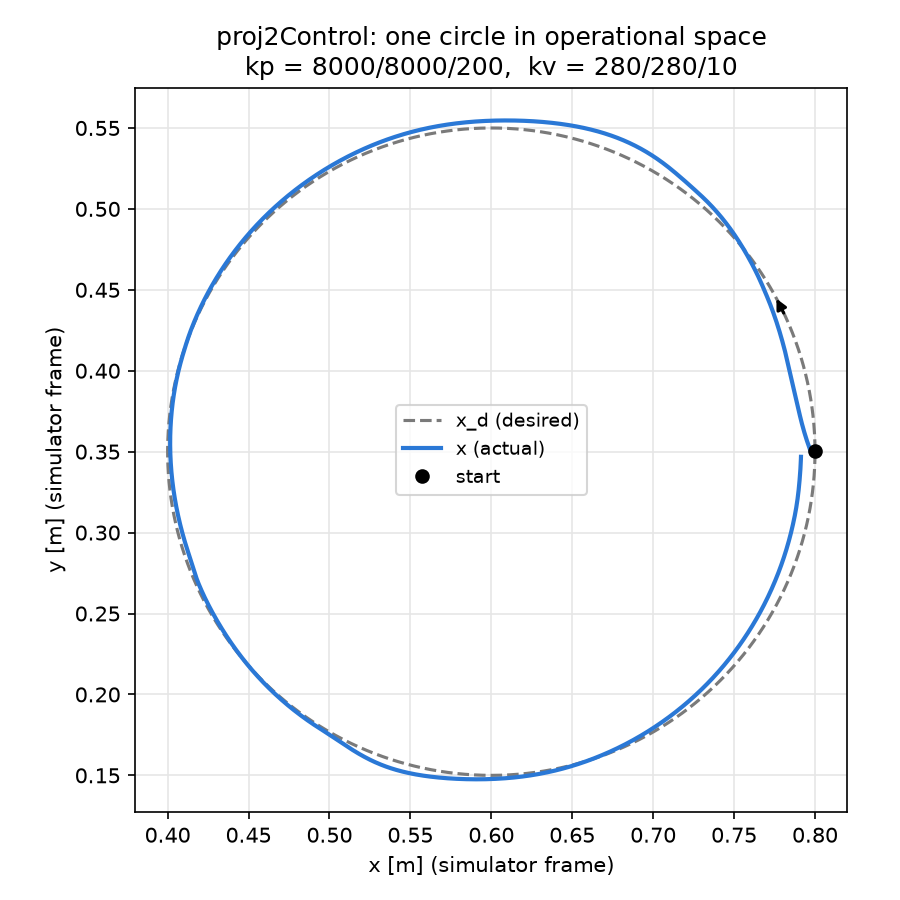
\includegraphics[width=\textwidth]{proj2_xy.png}
\end{minipage}\hfill
\begin{minipage}[c]{0.61\textwidth}
\textbf{Gains:} $k_p = 8000/8000/200$, $k_v = 280/280/10$ for $(x, y, \alpha)$.

\textbf{Result:} position error always $< 11$\,mm, orientation $< 0.03$\,rad. Peaks $116 / 38 / 1$\,Nm (limits
$156.4 / 89.4 / 20.1$).

\textbf{Peak at the start:} the arm stands still, but $\dot x_d$ jumps from 0 to $r\dot\beta = 0.25$\,m/s. The D term
suddenly wants a large force. In the $x$-$y$ plot the end effector leaves the circle a bit right after the start.

\smallskip
{\small
\begin{tabular}{lccccc}
  \toprule
  $k_p$ ($x$, $y$) & 1000 & 2000 & 4000 & 8000 & 12000 \\
  \midrule
  RMS error [mm] & 47 & 26 & 14 & 7 & 5 \\
  \bottomrule
\end{tabular}
}
\end{minipage}

\textbf{Error $\sim 1/k_p$:} double $k_p$, half the error, the shape of the curve stays the same. Our explanation: the
controller is a spring between $x$ and $x_d$. To move along the circle the arm needs a certain force, and a spring with
stiffness $k_p$ has to be stretched by $e = F/k_p$ to give this force.

\textbf{Limits:} $k_p = 12000$ gives 5\,mm, but $146$\,Nm at joint 1, too close to $156.4$. We increased $k_v$ together
with $k_p$ so that nothing oscillates. A much larger $k_v$ does not work either: $k_v = 500$ gives $168$\,Nm because of
the velocity jump.

\sagen{The stiffer the spring $k_p$, the smaller the error, roughly $\propto 1/k_p$. The limit is the torque at joint 1.}

\begin{fragen}
\frage{How does the error change with $k_p$?}
{Roughly $\propto 1/k_p$: $47 \to 26 \to 14 \to 7$\,mm for $1000 \to 8000$. The shape stays, the curve only gets
smaller.}
\frage{What limits $k_p$ and $k_v$?}
{The torque limits, mainly at joint 1 (see above). A $k_v$ that is too small makes the end effector oscillate.}
\frage{Why is the largest peak right at the start?}
{The desired velocity jumps from 0 to 0.25\,m/s while the arm still stands. The D term sees a large error
$\dot x - \dot x_d$ and produces a large force. C4 fixes this.}
\end{fragen}

%=====================================================================
\section{C4: Parabolic blends (\code{proj3})}
%=====================================================================

\begin{herleitung}{parabolic blends for \texorpdfstring{$\beta$}{beta} (important)}
Three parts: blend with constant acceleration $\ddot\beta = \frac{2\pi}{25}$, linear part with
$\dot\beta = \frac{2\pi}{5}$, blend with constant deceleration down to 0.

\textbf{Blend time} (hint in the sheet): $\dot\beta(t_b) = t_b\,\ddot\beta = \frac{2\pi}{5}
\;\Rightarrow\; t_b = \frac{\dot\beta}{\ddot\beta} = \frac{2\pi/5}{2\pi/25} = 5$\,s.

\textbf{Total time:} angle in one blend $\frac12\ddot\beta\,t_b^2 = \frac12 \cdot \frac{2\pi}{25} \cdot 25 = \pi$. Three
circles are $\beta_f = 6\pi$. Both blends together $2\pi$, so $4\pi$ are left for the linear part, which takes
$4\pi / \frac{2\pi}{5} = 10$\,s. So $t_f = 5 + 10 + 5 = 20$\,s.
\[
  \beta(t) =
  \begin{cases}
    \frac12\ddot\beta\,t^2 & 0 \le t < t_b \\[2pt]
    \frac12\ddot\beta\,t_b^2 + \dot\beta\,(t - t_b) & t_b \le t < t_f - t_b \\[2pt]
    \beta_f - \frac12\ddot\beta\,(t_f - t)^2 & t_f - t_b \le t < t_f \\[2pt]
    \beta_f & t \ge t_f
  \end{cases}
  \qquad
  \dot\beta(t) =
  \begin{cases}
    \ddot\beta\,t \\[2pt]
    \dot\beta \\[2pt]
    \ddot\beta\,(t_f - t) \\[2pt]
    0
  \end{cases}
\]
The second blend is the first one mirrored, counted backwards from the end. The transitions are continuous: at $t_b$
$\beta = \pi$, at $t_f - t_b = 15$\,s $\beta = \pi + 4\pi = 6\pi - \pi = 5\pi$, and the velocity fits as well.
$\beta$ and $\dot\beta$ go into \code{setCircleTarget} from C1, controller as in C2.
\end{herleitung}

\begin{minipage}[t]{0.66\textwidth}
\vspace{0pt}
\begin{lstlisting}[firstnumber=531]
  double t = gv.curTime - circle_start_time;
  double acc = CIRCLE_ANGULAR_ACCELERATION;
  double vel = CIRCLE_ANGULAR_VELOCITY;
  double tb = vel / acc;
  double tf = CIRCLE_TOTAL_ANGLE / vel + tb;

  double beta, dbeta;
  if (t < tb) {
    beta = 0.5 * acc * t * t;
    dbeta = acc * t;
  } else if (t < tf - tb) {
    beta = 0.5 * acc * tb * tb + vel * (t - tb);
    dbeta = vel;
  } else if (t < tf) {
    // mirror image of blend 1, measured backwards from the end
    double t_left = tf - t;
    beta = CIRCLE_TOTAL_ANGLE - 0.5 * acc * t_left * t_left;
    dbeta = acc * t_left;
  } else {
    beta = CIRCLE_TOTAL_ANGLE;
    dbeta = 0.0;
  }

  setCircleTarget(gv, beta, dbeta);
  operationalSpaceControl(gv);
\end{lstlisting}
\end{minipage}\hfill
\begin{minipage}[t]{0.32\textwidth}
\vspace{0pt}
\centering
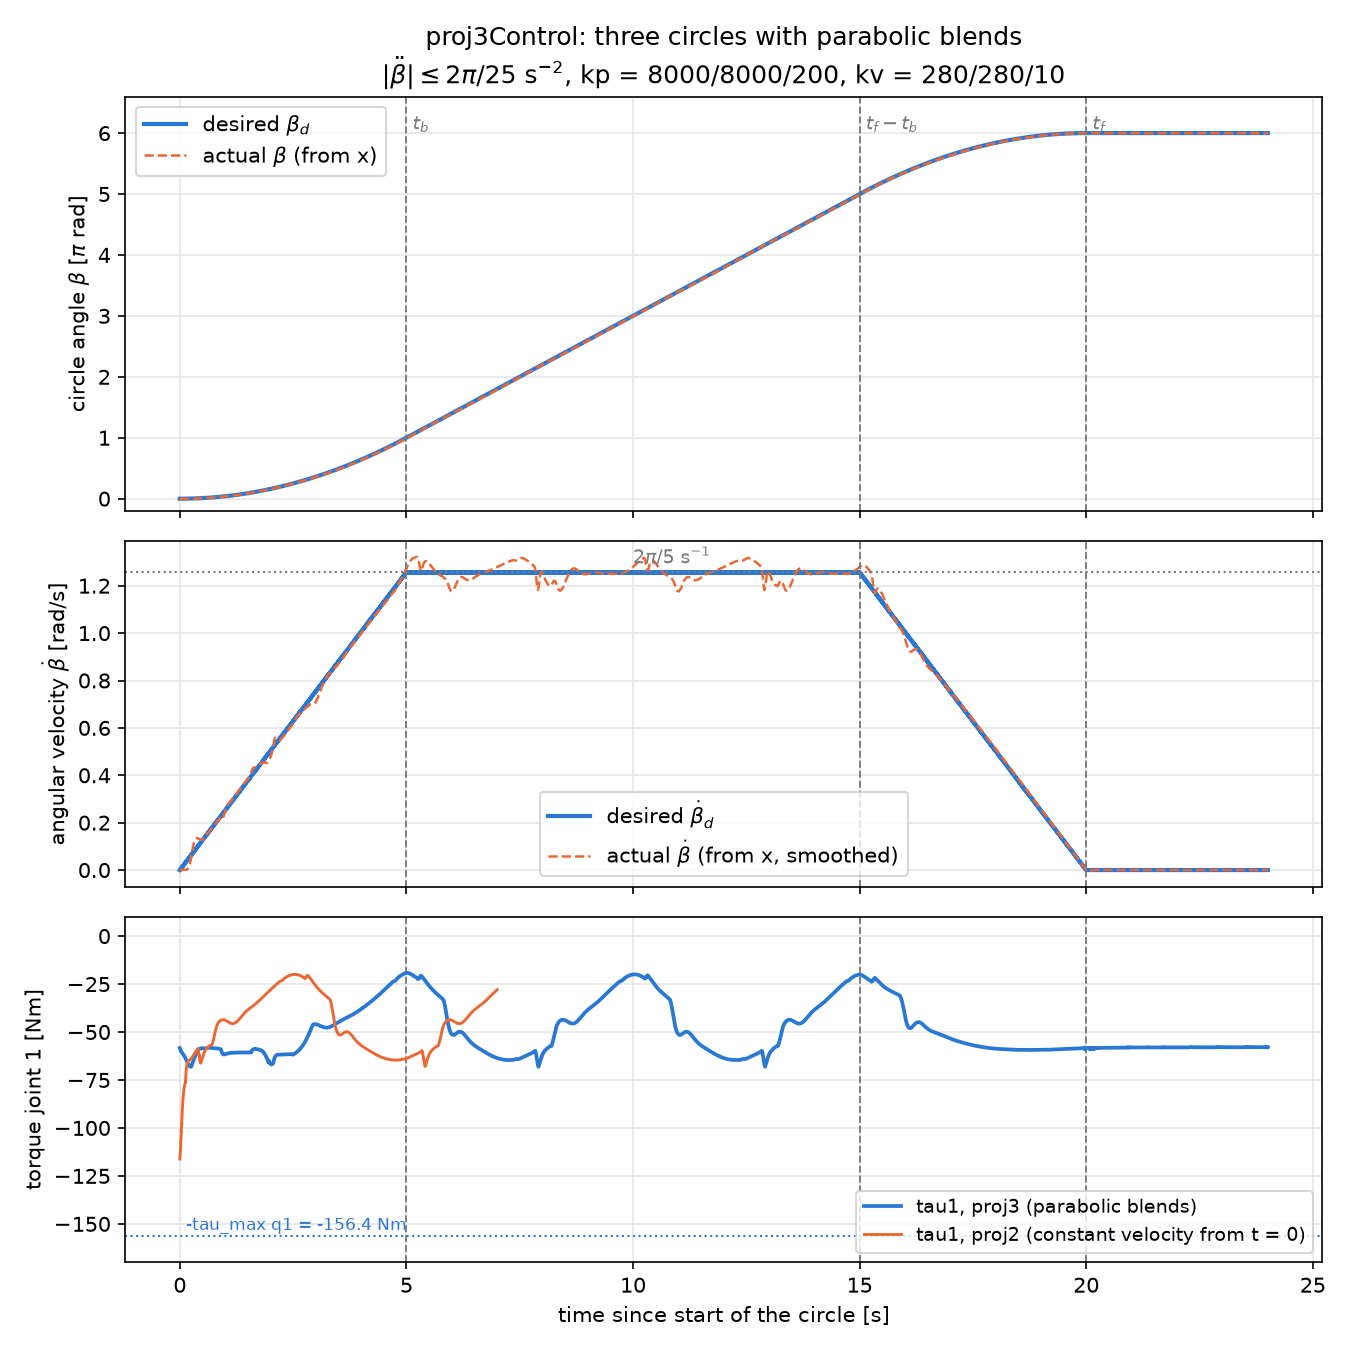
\includegraphics[width=\textwidth]{proj3_blends.png}
\end{minipage}

\textbf{L.\,108--109:} $\ddot\beta = 2\pi/25$, $\beta_f = 3 \cdot 2\pi$. \textbf{L.\,534--535:} $t_b$ and $t_f$ are
computed, not typed in. $t_f = \beta_f/\dot\beta + t_b = 15 + 5 = 20$\,s is the same as $2t_b + 4\pi/\dot\beta$, because
$2 \cdot \frac12\ddot\beta t_b^2 / \dot\beta = t_b$. \textbf{L.\,538--552:} the four cases of the formula.

\textbf{Result:} same gains as proj2. Error again $< 11$\,mm, no peak at the start any more: max.\ $68$\,Nm at joint 1
instead of $116$\,Nm with proj2. After 20\,s ($\beta = 6\pi$, $\dot\beta = 0$) the end effector holds the end point, which
is the start point $(0.8,\ 0.35)$ again.

\sagen{Instead of starting at full speed, $\beta$ accelerates evenly for 5\,s, moves at constant speed for 10\,s and brakes
for 5\,s. So the desired velocity never jumps, and the torque peak at the start is gone.}

\begin{fragen}
\frage{Why parabolic blends?}
{In proj2 the desired velocity jumps at the start (and when stopping). With limited acceleration it rises linearly,
there is no jump and no torque peak any more.}
\frage{How do you get $t_b$ and $t_f$?}
{$t_b$: at the end of the blend the velocity has to be $\frac{2\pi}{5}$, so $t_b \cdot \frac{2\pi}{25} = \frac{2\pi}{5}$,
$t_b = 5$\,s. $t_f$: each blend covers $\pi$, $4\pi$ are left for the linear part, that is $10$\,s, in total $20$\,s.}
\frage{Is the acceleration limit kept?}
{Yes. In the blends $|\ddot\beta| = \frac{2\pi}{25}$, exactly at the limit, in the linear part it is 0.}
\end{fragen}

%=====================================================================
\section{C5: Bonus}
%=====================================================================

For the bonus we used controllers of the template that were free otherwise, so everything stays in \code{control.cpp}.
All of them use the controller from C2, the gains of proj2 and the same path speed $0.25$\,m/s, starting at the circle
start.

\begin{minipage}[c]{0.5\textwidth}
\begin{itemize}
  \item \code{lineControl}: line $(0.8, 0.35) \leftrightarrow (0.4, 0.35)$, back and forth.
  \item \code{xtrackControl}: square, side $0.2$\,m, counter-clockwise like the circle.
  \item \code{nxtrackControl}: circle + noise, random $\pm 10\,\%$ of $\tau_{\max}$ in every cycle.
  \item \code{ntrackControl}: circle, but only $80\,\%$ of $G$.
\end{itemize}
\end{minipage}\hfill
\begin{minipage}[c]{0.47\textwidth}
\centering
{\small
\begin{tabular}{lccc}
  \toprule
  Path & max. & RMS & max.\ $|\tau_1|$ \\
  \midrule
  Circle & 11\,mm & 7\,mm & 116\,Nm \\
  Line & 22\,mm & 9\,mm & 99\,Nm \\
  Square & 50\,mm & 19\,mm & 138\,Nm \\
  \bottomrule
\end{tabular}
}
\end{minipage}

\secneed{8\baselineskip}
\begin{lstlisting}[firstnumber=445]
void nxtrackControl(GlobalVariables& gv)
{
  bonusCircle(gv);
  for (int i = 0; i < gv.dof; i++) {
    gv.tau[i] += NOISE_RATIO * gv.taumax[i] * randomUnit();
  }
}
\end{lstlisting}
\textbf{L.\,445--451:} first the normal circle (\code{bonusCircle}, l.\,225--230), then a random value between $-10\,\%$
and $+10\,\%$ of $\tau_{\max}$ is added to every torque. \code{randomUnit} (l.\,218--222) is a simple random number
generator of our own, so no extra include is needed; the fixed start value gives the same noise in every run.
\textbf{L.\,482--486:} \code{ntrackControl} also computes the normal circle first and then subtracts
\code{gv.G * (1.0 - GRAVITY\_COMPENSATION\_RATIO)}, so $\tau = J^T F + G - 0.2\,G = J^T F + 0.8\,G$.

\textbf{Results (compared with the normal circle):}
\begin{itemize}
  \item \textbf{What the plot shows:} the distance to the normal run, not the tracking error $|x - x_d|$. The tracking error hardly changes: RMS $7.1$ (noise) and $7.3$ ($G$) instead of $7.2$\,mm.
  \item \textbf{Noise:} on average only $0.7$\,mm (after the start max.\ $1.6$\,mm), although up to $15.6$\,Nm at joint 1. The noise is
        different in every cycle and zero on average. The heavy arm cannot follow such fast changes, and the controller
        corrects the rest.
  \item \textbf{80\,\% of $G$:} on average $2.6$\,mm (max.\ $3.9$\,mm). The missing torque is always there and always acts
        in the same direction. The P term has to replace it, and for that it needs an error.
  \item \textbf{Not the same everywhere:} with the $G$ error the deviation changes along the circle (after the start offset of $1.3$\,mm, the recordings do not start at exactly the same point) between $1.7$ and
        $3.9$\,mm. It is large where $|\det J|$ is small ($0.10$--$0.12$, closer to a singularity), and small where
        $|\det J|$ is large ($0.16$--$0.18$). Our explanation: through $\tau = J^T F$ the controller needs a larger force
        for the same torque close to a singularity, and a larger force means a larger error. Also the missing torque
        itself depends on the pose.
\end{itemize}

\sagen{Smooth paths are easy, jumps in the velocity are hard. Noise averages out, a constant model error does not, and
how strong it acts depends on the pose.}

\begin{fragen}
\frage{Which paths are easy, which are hard, and why?}
{Easy: smooth paths like the circle, the velocity changes its direction slowly. Hard: jumps in the velocity, so the
turning points of the line ($-0.25 \to +0.25$\,m/s) and the corners of the square (quarter turn). These would need
infinite acceleration, the arm overshoots, and the D term gives a peak. On the straight parts line and square are as good
as the circle. Same effect as proj2 vs.\ proj3.}
\frage{Why does noise disturb less than a constant error?}
{Noise is zero on average and changes every cycle, the arm averages it out. A constant error in $G$ always pulls in the
same direction, and the P term has to make up for it with a steady error.}
\frage{Is the behaviour the same in the whole workspace?}
{No. The deviation depends on the pose: larger where $|\det J|$ is small, so closer to a singularity.}
\end{fragen}

%=====================================================================
\section{General questions (everyone has to be able to answer them)}
%=====================================================================

\begin{fragen}
\frage{Why C++98, no \code{new}, only static memory?}
{It is in the coding rules: the code should also run on the real Puma, on a real-time PC with QNX and a 500\,Hz control
loop. That is why we use e.g.\ the global variable \code{spline} instead of dynamic memory.}
\frage{Why no output (\code{printf}/\code{cout})?}
{Output takes too long and would disturb the control loop. \code{PrintDebug} of the template stays unchanged, it only
runs on the command \code{pdebug}.}
\frage{Where are the gains?}
{Never in the code, always \code{gv.kp}/\code{gv.kv}. Saved with ``Store gains'' in \code{gains\_1.txt} (\code{\_1} =
3-DOF mode), one block per controller: number of joints, $k_p$ row, $k_v$ row.}
\frage{Do you limit the torque in the code?}
{No, the sheet does not allow it. We tested with ``torque limits'' switched off and chose the gains so that the peaks stay
below $\tau_{\max}$ (proj1 $55.5$, proj2 $116$, proj3 $68$\,Nm at joint 1).}
\frage{Joint space or operational space -- pros and cons?}
{Joint space (part B): simple, no problems with singularities, but the end effector does not follow a given shape.
Operational space (part C): you can follow shapes like a circle, but there are problems close to singularities
(tutorial T5).}
\frage{Where does $G$ come from in A2?}
{From the simulator (\code{gv.G}), as the sheet asks. \code{PreprocessControl} no longer computes our model from A1.}
\end{fragen}

\end{document}
